\documentclass[11pt]{article}
\usepackage{amssymb}
\usepackage[UTF8]{ctex}
\usepackage{geometry}
\usepackage{units}
\usepackage{pifont}
\geometry{
	a4paper,
	total={150mm,237mm},
	left=30mm,
	top=27mm,
	}
\usepackage{amsmath}
\usepackage{enumerate}
\usepackage{lipsum}
\usepackage{graphicx}
\usepackage{hyperref}
\usepackage{indentfirst}
\usepackage[graphicx]{realboxes}
\usepackage{booktabs}
\usepackage{cases}
\usepackage{subfig}  
\usepackage{float}
\usepackage{pythonhighlight}

\setlength{\parindent}{2em}
\title{HW8}
\author{姓名:陈锐林,学号:21307130148}

\begin{document}
\maketitle
\begin{Large}
    \noindent Chapter 28\\
\end{Large}
Question1\par
(1)我理解了这段汇编。(2)这里的锁(acquire部分),是通过循环不断对一个变量判0,之后再下一步。\\
Question2\par
(1)按默认设置运行flag.s是没问题的;可以看到默认设置下,一共2个线程,并且线程中断达50,是远大于代码数的。(2)鉴于前面的信息,能看出两个线程会正常运行,最后flag会正常被清0;在利用-M,-R,-c后可验证属实。\\
Question3\par
(1)如果在前面的命令加上"-a bx=2,bx=2"对寄存器进行设置,flag仍然是0;因为设置bx=2,相当于让整个大循环运行两次。(2)如果想让flag最后不为1,应该是利用中断。比如下面这张图中,右侧线程2本来flag为1(-a bx=5,bx=4),但是中断后就变为0了。所以如果要在线程1达到这个目的,应该是在线程1最后一个循环对flag清零
后又跳到线程2,置1后再回来;但这后续是无法达到的,因为默认设置中thread interrupt有50,线程1结束时flag为1,但是很快就会切换到线程2,继续操作,最后flag总会被清零的。
\begin{figure}[H]
    \centering
    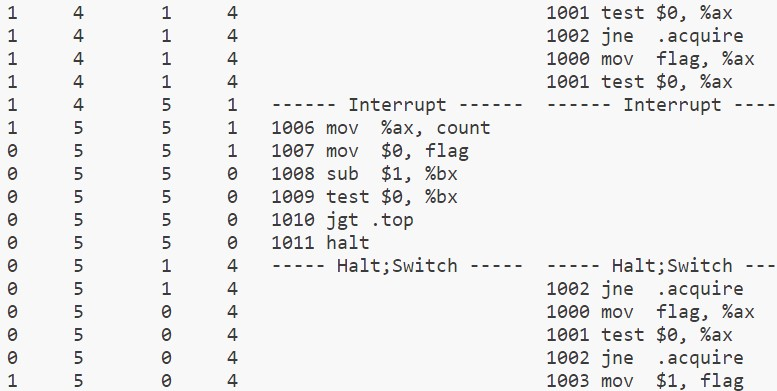
\includegraphics[height=8cm,width=10cm]{hw8-1.jpg}
\end{figure}
\newpage
\noindent Question4\par
(1)这题所谓的坏结果和好结果应该是针对count和ax的,因为第三题中我们已经知道flag固定为0结束。如这里让命令为 -a bx=10,bx=10;最后的count和ax应该都是20;但是事实上根据中断频率的不同会得到不同结果。
尝试了1-15的中断频率后,我发现只有11和15能得到好结果,其他都是坏结果。(2)尝试解释下原因:原因在mov count,\%ax / add \$1,\%ax / mov \%ax,count;这三句中间可能发生中断,最后count得到的ax值可能和之前相比没有增长。
而中断频率等于11,对应着完成一次大循环的代码数,所以不会有这个问题。而15也是正好避开了,如果再扩大bx可能会出问题。\\
Question5\par
(1)上锁是用的 xchg \%ax, mutex;这是一个原子操作,将ax和mutex中的值进行对换,并返回mutex的值。之后如果ax是0(mutex原本是0),就进行下一步;否则继续循环。(2)开锁就是将变量0给到mutex。\\
Question6\par
(1)仍然取bx=10,bx=10;考虑-i从1-15;可以看到最后得到的结果mutex都是0,是正确的。(2)而关于CPU的浪费问题,发现中断频率较小时总的指令数很大,比如取4时是306;而取11时就只有222。(该数据通过添加-S标志得到)。应该是因为锁的问题导致的循环步数增加,在中断频率低的时候就比较容易遇到。\\
Question7\par
采用命令如:python3 ./x86.py -p test-and-set.s -M mutex,count -R ax,bx -c -a bx=10,bx=10 -P 0011 , 就可以模拟题目中的情况。这段命令即thread0和thread1每两条交替运行;能观察到在0中的锁在1中被acquire;仅从mutex/ax/count的值来看是正确的。但是应该还要CPU的效率问题。\\
Question8\par
变量turn的存在保证了两个线程不会陷入竞争获得一个锁的死循环。这种情况下即使两个线程flag都是1了,也不会产生矛盾。\\
Question9\par
首先采取不同的-i并不会导致最后结果的不同(count flag cx ax保持一致)。唯一不同的可能是CPU的效率,发现从1-15,用指令最多的反而是-5和-6,达到50多条。\\
Question10\par
通过改变不同的执行序列,我们能观察结果是否正确。而在上面已经采用了不同的-i,所以这里选择用一些数量不均衡或者顺序不对称的-P即可。比如-P 010; -P 00001; -P 11011; -P 1001。在试验过程中,观察在线程切换前后是否有不正常行为发生;最后可以看到,
只有用的指令数的差别,而没有逻辑上的错误。\\
Question11\par
(1)ticket.s是一个ticket锁的定义和使用,和前文中的内容是对应的。(2)这里使用命令"python3 ./x86.py -p ticket.s -M count,ticket,turn -R ax,bx,cx -a bx=1000,bx=1000 -c",能看到最后得到的结果是正确的, count,ticket,turn=2000。如下图:
\newpage
\begin{figure}[h]
    \centering
    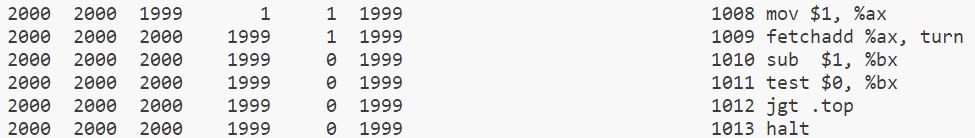
\includegraphics[height=3cm,width=10cm]{hw8-2.jpg}
\end{figure}
\noindent Question12\par
使用命令"python3 ./x86.py -p ticket.s -M count -t 6 -c -i 5",将线程增加到6个,会发现它们都陷入了.tryagain的循环,如下图的运行结果所示。
\begin{figure}[h]
    \centering
    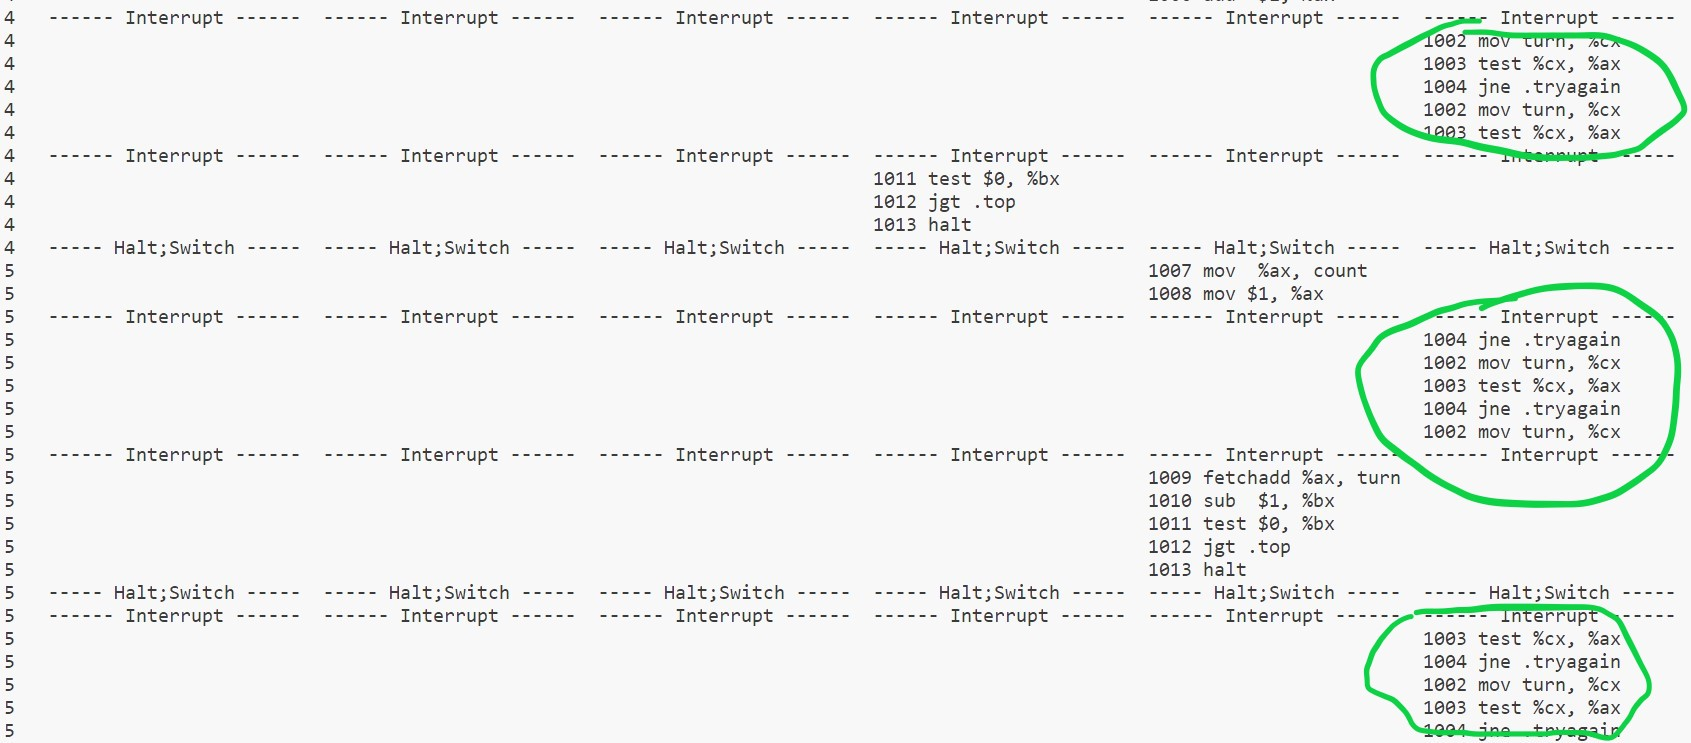
\includegraphics[height=8cm,width=10cm]{hw8-3.jpg}
\end{figure}\\
Question13\par
(1)使用以下两条命令:"./x86.py -p test-and-set.s -M count,mutex -R ax,bx -a bx=5,bx=5 -c -i 4 -S" 和 "./x86.py -p yield.s -M count,mutex -R ax,bx -a bx=5,bx=5 -c -i 4 -S"。前者用了190条指令,后者只用了156条节省34条。
(2)可以看到yield里主动让出时间片给其他线程,减少了自旋等待时间的;为了能更好地利用这个优势,我们可以在较多线程的时候使用yield。\\
Question14\par
(1)从名字上来看就知道,这个锁和test-and-set.S所作的是差不多的。只是在最前面添了三行代码:mov  mutex, \%ax / test \$0, \%ax / jne .acquire;意思就是不直接去进行xchg,而是先对ax判0。
(2)这样做能避免无意义的xchg,当且仅当锁空闲时才会更换mutex的值,从而提高效率。
\newpage
\begin{Large}
    \noindent Chapter 30\\
\end{Large}
Question1\par
查看后知道,这是通过单一条件变量来解决生产者/消费者问题。\\
Question2\par
这里我用了下面5条指令,这些是题目中参数的不同组合:\par
./main-two-cvs-while -p 1 -c 1 -m 1 -v;\par
./main-two-cvs-while -p 1 -c 1 -m 10 -v;\par
./main-two-cvs-while -p 1 -c 1 -m 10 -l 100 -v;\par
./main-two-cvs-while -p 1 -c 1 -m 1 -C 0,0,0,0,0,0,1 -v;\par
./main-two-cvs-while -p 1 -c 1 -m 10 -l 10 -C 0,0,0,0,0,0,1 -v;\par
(1)题目问代码的行为有没有随着缓存区变大而改变,有点没get到在问什么,应该是没有变化。(2)关于NF的变化,从第一条指令到第二条指令就能知道;只提升缓冲区大小是没法改变的,
NF都是0或者1;而从第二条指令到第三条指令又能看出,只改变生产者数量也不能改变NF;但是如果对比第四条和第五条指令就能知道,只要增加了睡眠时间,那么改变生产者和消费者数量就能改变NF分布;这里第五条指令下
NF会从0变化到10。\\
Question3\par
./main-two-cvs-while -p 1 -c 1 -m 10 -l 10 -C 0,0,0,0,0,0,1 -v在windows和linux上,得到结果是不一样的,如下:
\begin{figure}[h]
    \centering
    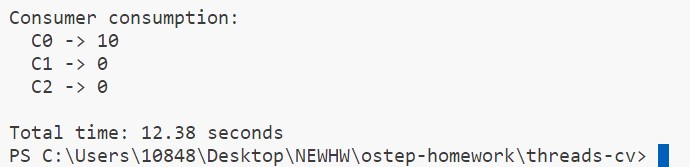
\includegraphics[height=4cm]{hw8-4.jpg}
\end{figure}
\begin{figure}[h]
    \centering
    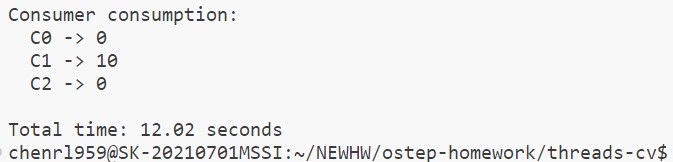
\includegraphics[height=4cm]{hw8-5.jpg}
\end{figure}
\\
Question4\par
根据题设,每个消费者会在获得锁之后睡眠1s,这时其他线程没法进行,所以在忽略其他时间计算下,总的时间就是c3的个数,即12s。
从具体的行为来看是这样的:c1消费第一个,无需等待;c0醒了之后,没法消费,等了1s后陷入沉睡;c2和c0类似;最后c0和c1共等9s,而最后三者各等1s。\\
Question5\par
改变-m的值为3,会导致总的c3步数为11,最后用时11s。可以看到,随着容量的增大,生产者不必等待EOS,这种情况发生了1次,节省了1s。\\
Question6\par
这题的命令和5相比只有睡眠时间点的差距。最后用时5s。是可以看到c6数量也是12,但是最后的时间不应该是12s,因为在解锁后睡眠,生产者可以继续进行,这样的情况占了7次。\\
Question7\par
还是用时5s,但是c6数量是13,但是仍能利用睡眠时间减去8s。\\
Question8\par
不可能,因为这里只有1个生产者和1个消费者。\\
Question9\par
可以的,采用以下命令:"./main-one-cv-while -c 2 -v -P 0,0,0,0,0,0,1"。如下,会看到c0进入等待后,一直在等待;最后出不来了。
\begin{figure}[h]
    \begin{center}
        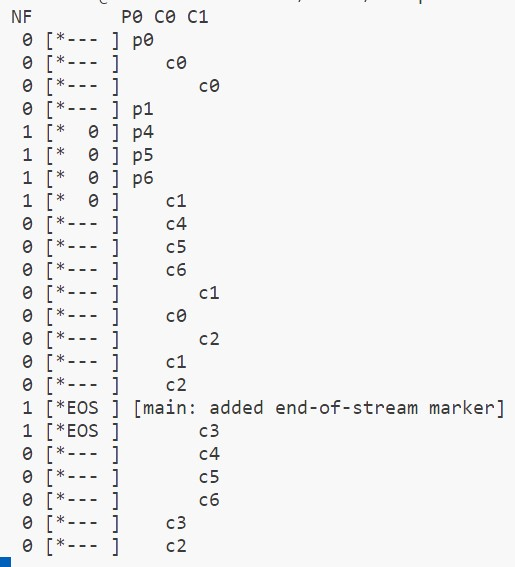
\includegraphics[height=8cm]{hw8-6.jpg}
    \end{center}
\end{figure}\\
Question10\par
1个消费者始终是正确的,两个之后就可能发生情况。c3准备,但是没有数据可以启动。\\
Question11\par
问题应该会出现在锁的提早释放导致同时进行do\_fill和do\_get操作。但是很可惜我这里没有找到能验证这个的命令。但还有其他问题,比如消费不均,这个命令很好找,如"./main-two-cvs-while-extra-unlock -p 1 -c 2 -m 10 -l 21 -v -C 0,0,0,0,1,0,0:0,0,0,0,0,0,0"即可。
\end{document}